
%(BEGIN_QUESTION)
% Copyright 2012, Tony R. Kuphaldt, released under the Creative Commons Attribution License (v 1.0)
% This means you may do almost anything with this work of mine, so long as you give me proper credit

\noindent
{\bf Programming Challenge and Comparison -- build a simple SCADA system} 

\vskip 10pt

``SCADA'' is an acronym meaning ``Supervisory Control And Data Acquisition'', referring to control systems where remote units relay data to and from a central location, allowing human operators to monitor and control processes spread over a wide area.  The term ``SCADA'' is broadly applied to many different types of control systems in industry.  Traditionally the term has been limited to control systems spread over a wide geographic area (e.g. power distribution systems, pipeline control systems) but it is now common to see ``SCADA'' used to describe {\it any} form of computer-based control system where process data is communicated over a digital network.  

\vskip 10pt

Work individually or in teams to wire and configure multiple PLC's to form a simple SCADA system, where analog data is read by a ``remote'' PLC and displayed by an HMI panel connected to a ``base'' PLC, and where virtual pushbuttons on the HMI display cause discrete outputs on the remote PLC to turn on and off.

$$\includegraphics[width=15.5cm]{i02799x01.eps}$$

When the potentiometer at the remote PLC is adjusted, the HMI at the base PLC should display a changing value.  When buttons on the HMI screen are toggled, indicator lamps at the remote PLC should turn on and off.  Feel free to include the following additional features for more fun and challenge:

\begin{itemize}
\item{} Build a ``trend graph'' display on the HMI instead of a simple numerical indicator for the analog input data point
\vskip 5pt
\item{} Have discrete inputs at the remote PLC register on the HMI display as graphic indicators
\vskip 5pt
\item{} Incorporate features such as input timers, event counts, etc. in the remote PLC
\vskip 5pt
\item{} Add multiple remote PLCs (use multi-drop RS-485 serial data communication, or Ethernet communication with a multi-port hub to connect the PLCs together)
\end{itemize}

\vskip 10pt

Successful completion of this system will require the use of analog scaling instructions as well as network messaging instructions.  All the usual caveats apply -- {\it have fun!}

\vfil 

\underbar{file i02799}
\eject
%(END_QUESTION)





%(BEGIN_ANSWER)

 
%(END_ANSWER)





%(BEGIN_NOTES)


%INDEX% PLC, I/O: analog resolution and scaling
%INDEX% PLC, ladder logic programming: analog input scaling
%INDEX% PLC, ladder logic programming: simple SCADA system

%(END_NOTES)


